% Author Vahid Partovi Nia
% Copyright Huawei Technologies
% Network Mind Team



\documentclass[12pt]{beamer}

\usetheme{Hannover}
\setbeamercolor{section in sidebar shaded}{fg=black}

\usecolortheme{beaver}
\beamertemplatenavigationsymbolsempty

%  \usebeamertemplate{navigation symbols}\hfill
%  \insertframenumber{}/\inserttotalframenumber}
  

\useoutertheme{sidebar}
\pgfdeclareimage[width=2.5\baselineskip]{institut-logo}{fig/mcgill_logo}
\setbeamertemplate{footline}
{\raisebox{-2ex}{\pgfuseimage{institut-logo}}
%  \hfill
\hspace{5cm}
  \usebeamertemplate{navigation symbols}
  \insertframenumber{}/\inserttotalframenumber
  \hspace{3.8cm}
YCBS255
}
%\setbeamertemplate{sidebar right}{}
  
\setbeamercolor{block title}{fg=darkred}
\setbeamercolor{local structure}{fg=darkred}

\setbeamercolor{palette sidebar secondary}{fg=darkgray, bg=white}



\usefonttheme{professionalfonts} % using non standard fonts for beamer


\makeatletter
\beamer@nav@subsectionstyle{hide/hide/hide}
\makeatother

\titlegraphic{
\includegraphics[width=2cm]{fig/mcgill_logo}}




\begin{document}

% no title and no author on sidebar
\title[]{Introduction to Statistical Learning}   
\author[]{Vahid Partovi Nia} 
\institute{YCBS  255: Applied Computational Statistics}
\date{23 October 2018} 


\makeatletter
  \begin{frame}[plain]
    \hspace*{-\beamer@leftsidebar}%
    \advance\textwidth by \beamer@leftsidebar\relax
    \beamer@leftsidebar=\z@
    \begin{minipage}{\textwidth}\par%
      \maketitle
    \end{minipage}
  \end{frame}
  \makeatother



\frame{\frametitle{Outline}\tableofcontents} 

\setbeamertemplate{sidebar left}[sidebar theme]



\section{Why?} 

\frame{\frametitle{Statistical Learning}
\begin{itemize}
\item Simple (predictive)
\item Interpretable (transparent box)
\item Fast to train (big data)
\item Works in wide variety of real problems (practical)
\item Easy to adapt (generalizable)
\item Building block of neural networks (deep learning)
\end{itemize}
}

\frame{\frametitle{Learning}
\begin{itemize}
\item $90\%$ Supervised learning: relate a predicting variable  $y$ to some other measured variables $x_j, j=1,\ldots, p$
\item $10\%$ Unsupervised learning:  data grouping using some measured variables $x$.
\end{itemize}
}

\frame{\frametitle{Why Python?}
\begin{itemize}
\item is popular
\item codes are readable
\item easy to learn
\item open source
\item combines machine learning with data analysis
\item many IDEs specially jupyter
\end{itemize}
}

\frame{
\url{http://github.com/vahidpartovinia/ycbs255}


\Huge
Introduction to Python
}

\section{Libraries}

\frame{\frametitle{Important libraries}
\begin{itemize}
\item numpy: arrays, linear algebra, random numbers, numerical methods.
\item pandas: data analysis, data visualization, data frames, statistics, basic statistical models.
\item matplotlib: plots and data visualization.
\item sklearn: machine learning algorithms.
\item scipy: advanced numerical methods (extended version of numpy).
\item statsmodels: advanced statistical models (extended version of pandas).
\end{itemize}
}

\frame{\frametitle{Schematic}
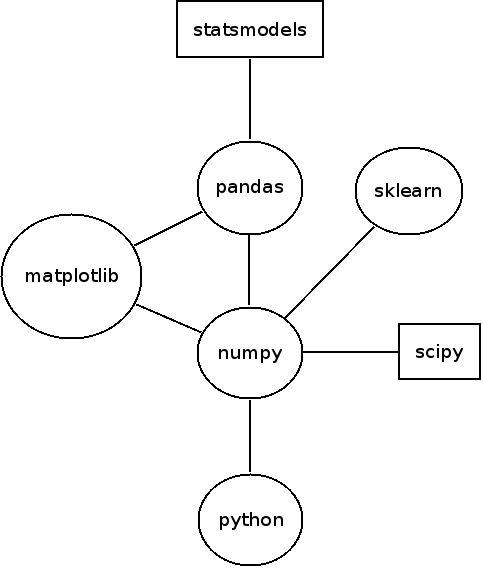
\includegraphics[width=0.5\textwidth]{fig/pylibs}
}


\frame{
\Huge Numpy
}


\frame{
\Huge Random vs Deterministic
}


\frame{\frametitle{Center as a predictor}
We are willing to predict sales
$$y_1= 22,\quad y_2 = 10, \quad y_3 = 9,\quad y_4 = 18$$
For prediction a probabilistic model is required.
$$y_i = \beta_0 + \varepsilon_i.$$
}



\frame{\frametitle{What is a good predictor?}
$$ y_1 = 22, \quad y_2 = 10, \quad y_3 = 9, \quad y_4 = 18 $$
\begin{center}
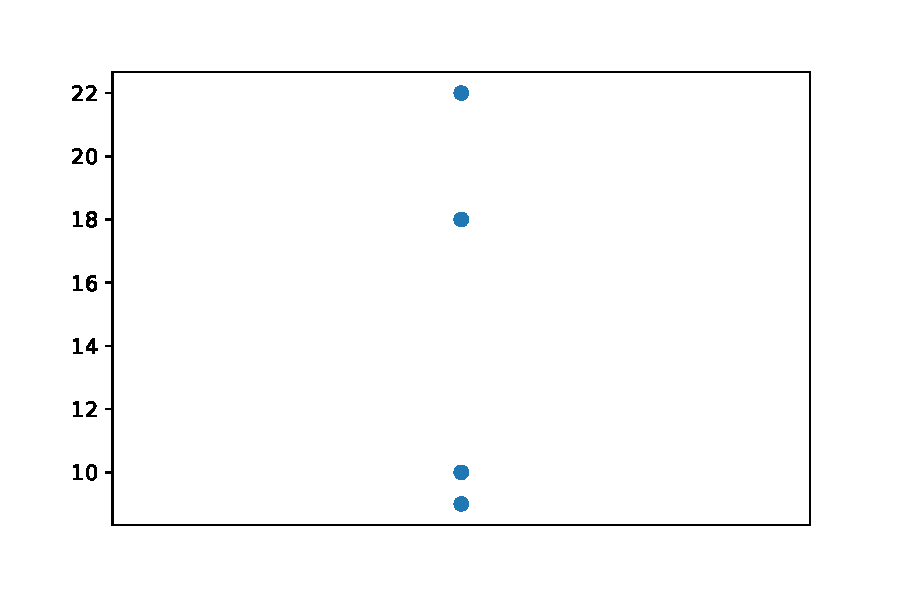
\includegraphics[width=0.5\textwidth]{fig/sales.pdf}
\begin{eqnarray*}
22 & =& \beta_0 + \varepsilon_1 \\
10 &= &\beta_0 + \varepsilon_2 \\
9  &= &\beta_0 + \varepsilon_3 \\
18 & =& \beta_0 + \varepsilon_4 \\
\end{eqnarray*}
\end{center}
}


\frame{\frametitle{Scale and location}
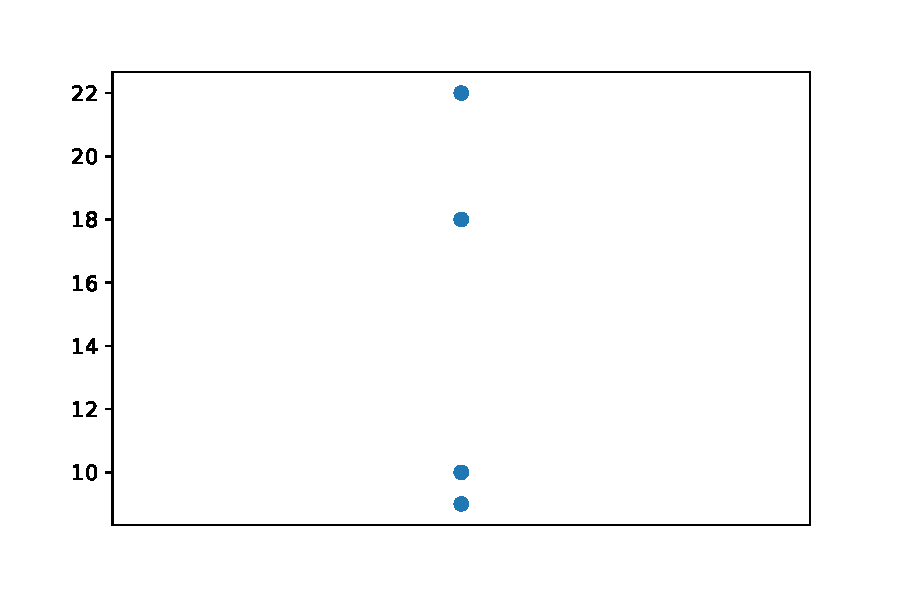
\includegraphics[width=0.5\textwidth]{fig/sales}
\begin{eqnarray*}
S_1(\beta_0) &=& {1\over n} \sum_{i=1}^n (y_i -\beta_0)^2 \\
S_2(\beta_0) &=&  {1\over n} \sum_{i=1}^n |y_i - \beta_0|
\end{eqnarray*}
}

\frame{\frametitle{What is mean?}
\begin{eqnarray*}
4 S_1(\beta_0) &=& (22 - \beta_0)^2 + (10 - \beta_0)^2 \\
&& + (9 - \beta_0)^2 + (18 - \beta_0)^2  \\
{d S_1(\beta_0) \over d \beta_0}& = & -2 (22 - \beta_0) -2(10 -\beta_0)\\
&&  -2(9-\beta_0) -2(18-\beta_0) =0 \\ \pause
\beta_0 &=&{1\over 4} (22 + 10+ 9 +18)
\end{eqnarray*}
}



\begin{verbatim}
> (22+10+9+18)/4
14.75


> import numpy as np
> y = np.array([22, 10, 9, 18])
> np.mean(y)
14.75
\end{verbatim} 
Which one?


\frame{
\Huge Matplotlib Pandas
}





%\frame{\frametitle{}
%}


\end{document}
